\chapter{Capacitancia y dieléctricos}
Un capacitor es un dispositivo que almacena energía potencial \textit{eléctrica} y carga eléctrica. Para hacerlo, basta aislar dos conductores uno del otro. Para almacenar energía en este dispositivo hay que transferir carga de un conductor al otro, de manera que uno tenga carga negativa y en el otro haya una cantidad igual de carga positiva. Debe realizarse trabajo para trasladar las cargas a través de la diferencia de potencial resultante entre los conductores, y el trabajo efectuado se almacena como energía potencial eléctrica.

Para un capacitor en particular, la razón entre la carga de cada conductor y la diferencia de potencial entre los conductores es una constante llamada \textit{capacitancia} \textbf{...}

\section{Capacitores y capacitancia}
Dos conductores separados por un aislante (o vacío) constituyen un \textbf{capacitor}. En la mayoría de las aplicaciones prácticas, cada conductor tiene inicialmente una carga neta cero, y los electrones son transferidos de un conductor al otro; a esta acción se le denomina \textit{cargar} el capacitor. Entonces, los dos conductores tienen cargas de igual magnitud y signo contrario, y la carga \textit{neta} en el capacitor en su conjunto permanece igual a cero. Cuando se dice que un capacitor tiene carga $Q$, o que una carga $Q$ está \textit{almacenada} en el capacitor, significa que el conductor con el potencial más elevado tiene carga $+Q$ y el conductor con el potencial más bajo tiene carga $-Q$ (si se supone que $Q$ es positiva). En los diagramas de circuito, un capacitor se representa con cualquiera de estos símbolos:

\begin{figure}[h]
\centering

\includegraphics[scale=0.4]{fig/capacitor}
\end{figure}

En cada uno de estos símbolos, las líneas verticales (rectas o curvas) representan los conductores, y las líneas horizontales representan los alambres conectados a uno y otro conductor. Una manera común de cargar un capacitor es conectar estos dos alambres a las terminales opuestas de una batería. Una vez establecidas las cargas $Q$ y $-Q$ en los conductores, se desconecta la batería. Esto da una \textit{diferencia de potencial} fija $V_{ab}$ entre los conductores (el potencial del conductor con carga positiva $a$ con respecto al potencial del conductor con carga negativa $b$), que es exactamente igual al voltaje de la batería.

El campo eléctrico en cualquier punto de la región entre los conductores es proporcional a la magnitud $Q$ de carga en cada conductor. Por lo tanto, la diferencia de potencial $V_{ab}$ entre los conductores también es proporcional a $Q$. La \textit{razón} entre la carga y la diferencia de potencial no cambia. Esta razón se llama \textbf{capacitancia} $C$ del capacitor:

\begin{equation}\label{24.1}\marginnote{Definición de capacitancia}
\boxed{C=\frac{Q}{V_{ab}}}
\end{equation}

La unidad del SI para la capacitancia es el \textbf{farad} (1\, F)

Cuanto mayor es la capacitancia $C$ de un capacitor, mayor será la magnitud $Q$ de la carga en el conductor de cierta diferencia de potencial dada $V_{ab}$, y, por lo tanto, mayor será la cantidad de energía almacenada. \textit{La capacitancia es una medida de la aptitud (capacidad) de un capacitor para almacenar energía}. El valor de la capacitancia sólo depende de las formas y los tamaños de los conductores, así como de la naturaleza del material aislante que hay entre ellos. 

\subsection{Cálculo de capacitancia: capacitores con vacío}
Se considerarán \textit{capacitores con vacío}; es decir, se supondrá que los conductores que constituyen el capacitor están separados por un espacio vacío.

La forma más sencilla de un capacitor consiste en dos placas conductoras paralelas, cada una con área $A$, separadas por una distancia $d$ que es pequeña en comparación con sus dimensiones (figura \ref{fig:cap-1}).

\begin{figure}[t]
\centering
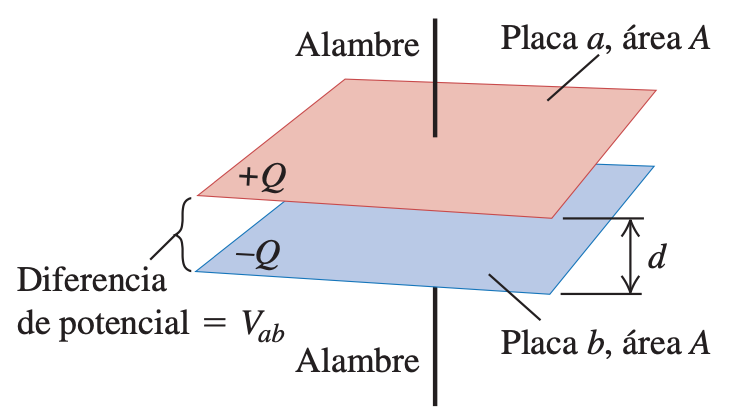
\includegraphics[scale=0.4]{fig/cap-placas-paralelas-1}
\caption{Arreglo de las placas del capacitor}
\label{fig:cap-1}
\end{figure}

\begin{figure}[t]
\centering
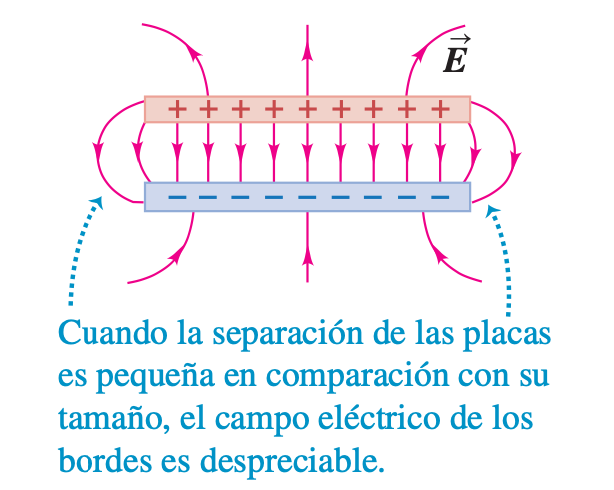
\includegraphics[scale=0.4]{fig/cap-placas-paralelas-2}
\caption{Vista lateral del campo eléctrico $\vec{E}$}
\label{fig:cap-2}
\end{figure}

Cuando las placas tienen carga, el campo eléctrico está localizado casi por completo en la región entre las placas (figura \ref{fig:cap-2}), el campo entre esas placas es esencialmente uniforme, y las cargas en las placas se distribuyen de manera uniforme en sus superficies opuestas. Este arreglo recibe el nombre de \textbf{capacitor de placas paralelas}.

Haciendo los cálculos, se sabe que, para este arreglo, la magnitud del cámpo eléctrico está dada por $E=\sigma/\epsilon_0$, donde $\sigma$ es la magnitud de la densidad superficial de carga en cada placa, es decir, $\sigma=Q/A$, por lo que se puede expresar como

\begin{equation*}
E=\frac{\sigma}{\epsilon_0}=\frac{Q}{\epsilon_0A}
\end{equation*}

El campo es uniforme y la distancia entre las placas es $d$, por lo que la diferencia de potencial (voltaje) es

\begin{equation*}
V_{ab}=Ed=\frac{1}{\epsilon_0}\frac{Qd}{A}
\end{equation*}

A partir de esto se observa que la capacitancia $C$ de un capacitor de placas paralelas con vacío es

\begin{equation}\label{24.2}\marginnote{Capacitancia de un capacitor de placas paralelas con vacío}
\boxed{C=\frac{Q}{V_{ab}}=\epsilon_0\frac{A}{d}}
\end{equation}

Notar que la capacitancia sólo depende de la geometría del capacitor. Cuando hay materia entre las placas, sus propiedades afectan la capacitancia.

\section{Capacitores en serie y en paralelo}
\subsection{Capacitores en serie}

\begin{figure}[h]
\centering
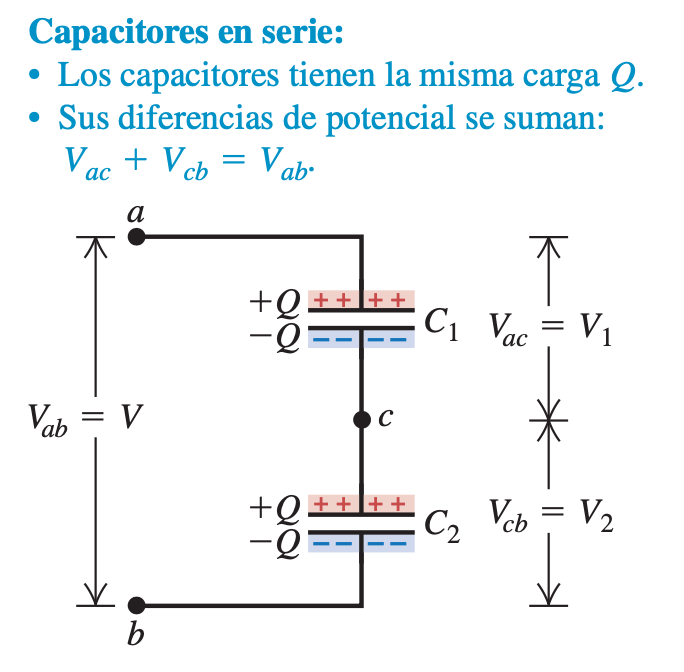
\includegraphics[scale=0.4]{fig/cap-serie-1}
\caption{Dos capacitores en serie}
\label{fig:cap-serie-1}
\end{figure}

\begin{figure}[h]
\centering
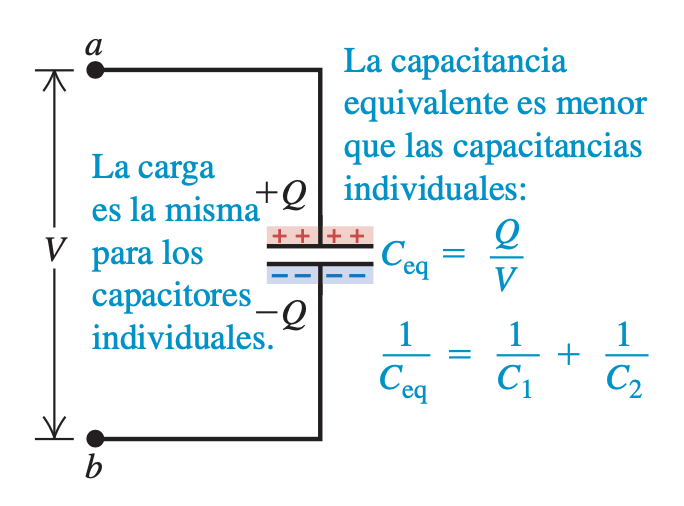
\includegraphics[scale=0.4]{fig/cap-serie-2}
\caption{El capacitor esquivalente único}
\label{fig:cap-serie-2}
\end{figure}

Se conectan en serie dos capacitores (uno en seguida del otro) mediante alambres conductores entre los puntos $a$ y $b$ (figura \ref{fig:cap-serie-1}).

\begin{equation}\label{24.5}\marginnote{Capacitores en serie}
\boxed{\frac{1}{C_{eq}}=\frac{1}{C_1}+\frac{1}{C_2}+\frac{1}{C_3}+\cdots}
\end{equation}

\begin{quote}
El recíproco de la capacitancia equivalente de una combinación en serie es igual a la suma de los recíprocos de las capacitancias individuales.
\end{quote}

\subsection{Capacitores en paralelo}
\begin{equation}\label{Capacitores en paralelo}\marginnote{Capacitores en paralelo}
\boxed{C_{eq}=C_1+C_2+C_3+\cdots}
\end{equation}

\begin{quote}
La capacitancia equivalente de una combinación en paralelo es igual a la suma de las capacitancias individuales.
\end{quote}

\section{Almacenamiento de energía en capacitores y energía de campo eléctrico}
La energía potencial eléctrica almacenada en un capacitor cargado es exactamente igual a la cantidad de trabajo requerido para cargarlo, es decir, para separar cargas opuestas y colocarlas en los diferentes conductores.

Suponga que cuando se carga el capacitor, la carga final es $Q$ y la diferencia de potencial final es $V$. Según la ecuación \ref{24.1}, estas cantidades están relacionadas de la siguiente forma $$V=\frac{Q}{C}$$

Sean $q$ y $v$ la carga y la diferencia de potencial, respectivamente, en una etapa intermedia del proceso de carga; entonces, $v=q/C$. En esta etapa, el trabajo $dW$ que se requiere para transferir un elemento adicional de carga $dq$ es $$dW=v\, dq=\frac{q\, dq}{C}$$

El trabajo total $W$ necesario para incrementar la carga $q$ del capacitor, de cero a un valor final $Q$, es

\begin{equation}\label{24.8}\marginnote{Trabajo para cargar el capacitor}
W=\int_0^WdW=\frac{1}{C}\int_0^Qq\, dq=\frac{Q^2}{2C}
\end{equation}

Si se define la energía potencial de un capacitor sin carga como igual a cero, entonces $W$ en la ecuación \ref{24.8} es igual a la energía potencial $U$ del capacitor con carga. La carga final almacenada es $Q=CV$, por lo que $U$ (que es igual a $W$) se expresa como

\begin{equation}\label{24.9}\marginnote{Energía almacenada en un capacitor}
\boxed{U=\frac{Q^2}{2C}=\frac{1}{2}CV^2=\frac{1}{2}QV}
\end{equation}

\subsection{Energía del campo eléctrico}
Debemos encontrar la energía por unidad de volumen en el espacio entre las placas paralelas de un capacitor con área $A$ y separación $d$. Ésta se denomina \textbf{densidad de energía} ($u$). De ecuación \ref{24.9}

\begin{equation}\label{24.10}
u=\frac{\frac{1}{2}CV^2}{Ad}
\end{equation}

De \ref{24.2} $C=\epsilon_0A/d$ y $V=Ed$. Reemplazando en \ref{24.10}

\begin{equation}\label{24.11}\marginnote{Densidad de energía eléctrica en vacío}
\boxed{u=\frac{1}{2}\epsilon_0E^2}
\end{equation}































